\documentclass[tocnosub,noragright,centerchapter,fullpagesingle,12pt]{uiuc_csthesis18}

% Updated version of the ECE department's latex resources

% Use draftthesis for notes and date markings on every page.  Useful when you
%   have multiple copies floating around.
% Use offcenter for the extra .5 inch on the left side. Needed with fullpage and fancy.
% Use mixcasechap for compatibility with hyperref package, which does NOT like all caps default
% Use edeposit for the adviser/committee on the title page.
% Use tocnosub to suppress subsection and lower entries in the TOC.
% PhD candidates use "proquest" for the proquest abstract.

\makeatletter

\usepackage{setspace}
\usepackage{epsfig}  % for figures
%\usepackage{graphicx}  % another package that works for figures
%\usepackage{subfigure}  % for subfigures
\usepackage{amsmath}  % for math spacing
%\usepackage{amssymb}  % for math spacing
%\usepackage{url}  % Hyphenation of URLs.
\usepackage{lscape}  % Useful for wide tables or figures.
%% Custom Packages
\usepackage[T1]{fontenc}
\usepackage{listings}
\usepackage{color}
\usepackage{xspace}
\usepackage[title]{appendix}
%\usepackage{tikz}
%\usepackage{pgf-pie}
\usepackage{forest}
\usepackage{amsmath,amssymb}
\usepackage{ctable}
\usepackage[textsize=tiny]{todonotes}
\usepackage{pifont}
\usepackage{calculator}
\usepackage{csquotes}
%\usepackage[ruled,vlined]{algorithm2e}
%\usepackage{algorithm}
%\usepackage{algorithmic}
\usepackage[linesnumbered,ruled]{algorithm2e}

% opphans
\clubpenalty = 10000
\widowpenalty = 10000
\displaywidowpenalty = 10000

%\setlength{\parskip}{0.5pt plus 4pt minus 3pt}
%\setlength{\textfloatsep}{1\baselineskip plus 0.2\baselineskip minus 0.5\baselineskip}
\newenvironment{tightcenter}{%
    \setlength\topsep{4pt}
    \setlength\parskip{-2pt}
    \begin{center}
    }{%
    \end{center}
}

% FIXME: overleaf broken if uncommented
\usepackage{tikz}
\usetikzlibrary{shapes,arrows,shadows,backgrounds}
\usetikzlibrary{arrows.meta}
\usepackage{amsmath,bm,times}

%% Custom Commands
\def\Code#1{\texttt{#1} }
%\def\Comment#1{}
\def\Comment#1{\textbf{\textsl{\color{red}  $\langle\!\langle$#1$\rangle\!\rangle$}} }
\newcommand{\percentage}[2]{\DIVIDE{#1}{#2}{\duv}\MULTIPLY{\div}{100}{\res}$\res\%$}
\newcommand{\revisit}[1]{{\color{red} Sandeep: #1}}
\newcommand{\Qd}[1]{{\color{red} Daejun: #1}}
\newcommand{\Qt}[1]{{\color{red} Theo: #1}}
\newcommand{\BW}[1]{{\color{red} Borrowed: #1}}
\newcommand{\Added}[1]{{\color{red} #1}}
%\newcommand{\SC}[1]{{\color{blue} #1}}
%\newcommand{\AEC}[1]{{\color{blue} #1}}
\newcommand{\SC}[1]{#1}
\newcommand{\AEC}[1]{#1}
\newcommand{\cmt}[1]{}
\newcommand{\xmark}{{\color{red} \ding{55}}}
\newcommand{\cmark}{{\color{green} \ding{51}}}
\newcommand{\ISA}{x86-64\xspace}
\newcommand{\LLVM}{LLVM IR\xspace}
\newcommand{\compd}{Compositional Lifter\xspace}
\newcommand{\siv}{single-instruction validation\xspace}
\newcommand{\Siv}{Single-instruction validation\xspace}
\newcommand{\plv}{program-level validation\xspace}
\newcommand{\tv}{translation validation\xspace}
\newcommand{\Mcstate}{\emph{State}\xspace}
%\newcommand{\K}{\mbox{$\mathbb{K}$}\xspace}
\newcommand{\Z}{$\mathbb{Z}3$\xspace}
\newcommand{\mcsema}{McSema\xspace}
\newcommand{\dlifted}{McSema-lifted\xspace}
\newcommand{\uif}{uninterpreted functions}
\newcommand{\TV}{Translation Validation\xspace}
\newcommand{\syncps}{synchronization points\xspace}
\newcommand{\syncp}{synchronization point\xspace}
\newcommand{\Strata}{Strata\xspace}
\newcommand{\Stoke}{Stoke\xspace}
\newcommand{\initS}{{\tt initial search}}
\newcommand{\secS}{{\tt secondary searches}}
%\newcommand{\K}{\ensuremath{\mathcal{{\tt K}}}\xspace}
\newcommand{\TS}[1]{{\tt #1}}
\newcommand{\matcher}{Matcher\xspace}
%\newcommand{\instr}[1]{\texttt{#1}}
\newcommand{\instr}[1]{\textbf{\color{brown}\m{#1}}}
\newcommand{\reg}[1]{\texttt{\%#1}}
\newcommand{\mem}[2]{\texttt{#1(\%#2)}}
\newcommand{\opcode}[1]{\ensuremath{#1}}
%\newcommand{\cond}[1]{\ensuremath{#1}}
\newcommand{\extract}{\emph{extract}\xspace}
\newcommand{\extractMInt}{\emph{extractMInt}\xspace}
\newcommand{\false}{\textbf{False}}
\newcommand{\true}{\textbf{True}}
\newcommand{\bool}{\texttt{Bool}\xspace}
\newcommand{\incfig}[1]{\includegraphics[scale=.7]{#1}}
\newcommand{\CF}[2]{$\s{F}_{\s{#2}}^{\s{#1}}$}
%\newcommand{\GN}[2]{$G{[#2]}^{#1}$}
\newcommand{\udef}{\emph{undef}\xspace}
\newcommand{\bv}[2]{$#1\text{'}#2$\xspace}
%% Graph algo
\newcommand{\N}{\s{N}\xspace}
\newcommand{\NP}{\s{N$^\prime$}\xspace}

\newcommand{\T}{\s{T}\xspace}
\newcommand{\TP}{\s{T$^\prime$}\xspace}

\newcommand{\un}{$u$\xspace}
\newcommand{\vn}{$v$\xspace}
\newcommand{\up}{$u^\prime$\xspace}
\newcommand{\IN}{\s{I$_{N}$}\xspace}
\newcommand{\INP}{\s{I$_{N^\prime}$}\xspace}
\newcommand{\F}{\s{F}\xspace}
\newcommand{\FP}{\s{F$^\prime$}\xspace}
\newcommand{\FN}{\s{F$_{N}$}\xspace}
\newcommand{\FNP}{\s{F$_{N}^\prime$}\xspace}
\newcommand{\GN}{\s{G$_{\FN}$}\xspace}
\newcommand{\GNP}{\s{G$_{\FNP}$}\xspace}
\newcommand{\Ap}{\s{A$^\prime$}\xspace}
\newcommand{\Bp}{\s{B$^\prime$}\xspace}
\newcommand{\Dp}{\s{D$^\prime$}\xspace}
\newcommand{\Lp}{\s{L$^\prime$}\xspace}
\newcommand{\Np}{\s{N$^\prime$}\xspace}
\newcommand{\Sp}{\s{S$^\prime$}\xspace}
\newcommand{\Tp}{\s{T$^\prime$}\xspace}

\newcommand{\pot}{$\phi$\xspace}
\newcommand{\potp}{\s{$\phi^\prime$}\xspace}
\newcommand{\potpup}{$\phi^\prime$(\up)\xspace}
\newcommand{\potvup}{$\phi_{v}$(\up)\xspace}
\newcommand{\potu}{$\phi$(\un)\xspace}
\newcommand{\potup}{$\phi$(\up)\xspace}

%%

\newcommand{\rating}[1]{%
    \begin{tikzpicture}[x=1ex,y=1ex]
    \begin{scope}
    \clip (0,1) circle (1);
    \fill[black] (-1,0) rectangle (1,#1/50);
    \end{scope}
    \draw[black, thin, radius=1] (0,1) circle;
    \end{tikzpicture}%
}

% opentuning results
\newcommand{\avgPassLength}{$8$\xspace}

% Current Support
\newcommand{\currentIS}{$3155$\xspace}
\newcommand{\currentIntel}{$774$\xspace}
% Total
\newcommand{\totalIS}{$3736$\xspace}
\newcommand{\totalIntel}{$996$\xspace}
\newcommand{\dup}{$109$\xspace}
% Mcsema
\newcommand{\mcsemaIS}{$1922$\xspace}
%
\newcommand{\plvT}{$2348$\xspace}
\newcommand{\plvP}{$2189$\xspace}
%
\newcommand{\sivIS}{$1349$\xspace}
\newcommand{\sivExc}{$573$\xspace}
\newcommand{\sivFail}{$29$\xspace}
\newcommand{\sivTO}{$6$\xspace}
\newcommand{\FPRate}{$7\%$\xspace}
%
% Strata
\newcommand{\strataIS}{$1796$}
\newcommand{\strataIntel}{$466$}
\newcommand{\strataWithDupIS}{$1905$}
\newcommand{\strataRegVarIS}{$692$}
% Unsupported
\newcommand{\system}{$210$}
\newcommand{\Xmmx}{$336$}
\newcommand{\crypto}{$35$}

\newcommand{\strataPerc}{$47\%$} % 466/996 or  1905 / 3736
\newcommand{\goelPerc}{$33\%$} 
\newcommand{\sailPerc}{$15\%$} 
% Stoke disjoin from Strata
%\newcommand{\stokeIS}{$332$} % 262 + 15 + 9 + 46. ALso 332/3767 == 9%
% 1432(strata common) + 332
\newcommand{\stokeIS}{${\sim}1764$}
%\newcommand{\stokeExcPerc}{$9\%$}
% Strata stoke combined
%\newcommand{\strataPlusStokeIS}{$2237$} % 

%\newcommand{\unsupp}{$939$}

%%%%%% Immediates
%\newcommand{\ImmUg}{$146$} % 118 + 28
%\newcommand{\ImmTotal}{$308$}
%\newcommand{\ImmG}{$190$}

%%%%%%% Registers
%\newcommand{\RegTOTAL}{$1133$} % 1083 + 50
%\newcommand{\RegSTRAT}{$742$} % 692 + 50
%\newcommand{\RegSTOK}{$262$}
%\newcommand{\RegMAN}{$129$}

%%% toture status
\newcommand{\TortureTotal}{$1576$} %
\newcommand{\TortureExclude}{$6$} % 6 + 22
\newcommand{\TortureInclude}{$1548$}
\newcommand{\TortureUifsInstr}{$293$} % 134(all three jobs) +  48
\newcommand{\TortureUifs}{$35$}
\newcommand{\TortureCoverage}{$963$}
%%% Undef counts
\newcommand{\undefTotal}{$474$}
\newcommand{\undefIntel}{$32$}
\newcommand{\undefPerc}{$3$} %32/1000

\input{header.tex}
\input{macro.tex}

\usepackage{hyperref}
\hypersetup{
    colorlinks=true,
    linkcolor=blue,
    filecolor=magenta,      
    urlcolor=cyan,
    bookmarks=true,
}


\definecolor{codegreen}{rgb}{0,0.6,0}
\definecolor{codegray}{rgb}{0.5,0.5,0.5}
\definecolor{codepurple}{rgb}{0.58,0,0.82}
\definecolor{backcolour}{rgb}{0.95,0.95,0.92}
\usepackage{courier}

\lstdefinestyle{Bash}{
    language=Bash,                % choose the language of the code
    basicstyle=\footnotesize\ttfamily,       % the size of the fonts that are used for the code
    numbers=left,                   % where to put the line-numbers
    numberstyle=\tiny\color{codegray},      % the size of the fonts that are used for the line-numbers
    stepnumber=1,                   % the step between two line-numbers. If it is 1 each line will be numbered
    numbersep=5pt,                  % how far the line-numbers are from the code
    backgroundcolor=\color{white},  % choose the background color. You must add \usepackage{color}
    showspaces=false,               % show spaces adding particular underscores
    showstringspaces=false,         % underline spaces within strings
    showtabs=false,                 % show tabs within strings adding particular underscores
    frame=single,           % adds a frame around the code
    %tabsize=2,          % sets default tabsize to 2 spaces
    captionpos=b,           % sets the caption-position to bottom
    breaklines=true,        % sets automatic line breaking
    breakatwhitespace=false,    % sets if automatic breaks should only happen at whitespace
    escapeinside={\%*}{*)},          % if you want to add a comment within your code
    commentstyle=\color{gray},
    keywordstyle=\color{blue},
    morekeywords={andnq, jp, jz, movw, movq, xorq, orq, retq, pushw}
}

\lstdefinestyle{LLVM}{
       %language=C,
   %basicstyle=\footnotesize,      
   basicstyle=\scriptsize\ttfamily,
   backgroundcolor=\color{white},  % choose the background color. You must add 
   %\usepackage{color}
   showspaces=false,               % show spaces adding particular underscores
   showstringspaces=false,         % underline spaces within strings
   showtabs=false,                 % show tabs within strings adding particular 
   %underscores
   frame=single,           % adds a frame around the code
   %tabsize=2,          % sets default tabsize to 2 spaces
   captionpos=b,           % sets the caption-position to bottom
   breaklines=true,        % sets automatic line breaking
   breakatwhitespace=false,    % sets if automatic breaks should only happen at 
   %whitespace
   escapeinside={(*}{*)},          % if you want to add a comment within your 
   %code
   commentstyle=\color{gray},
   morecomment=[l]{;},
   keywordstyle=\color{blue},
   %morekeywords={regstate, stackmem, andBool, requires, ensures, codemem, 
   %memstate, and}
   morekeywords={andBool, requires, ensures, and, rule, type, getelementptr, 
       extract, add, if, then, else, fi, concat, define, internal, i64, 
       call,ret, store, load,global, zeroinitializer,i8}
}

\lstdefinestyle{LLVMWOBORDER}{
    %language=C,
    %basicstyle=\footnotesize,      
    basicstyle=\scriptsize\ttfamily,
    backgroundcolor=\color{white},  % choose the background color. You must add 
    %\usepackage{color}
    showspaces=false,               % show spaces adding particular underscores
    showstringspaces=false,         % underline spaces within strings
    showtabs=false,                 % show tabs within strings adding 
    %particular 
    %underscores
    %frame=single,           % adds a frame around the code
    %tabsize=2,          % sets default tabsize to 2 spaces
    captionpos=b,           % sets the caption-position to bottom
    breaklines=true,        % sets automatic line breaking
    breakatwhitespace=false,    % sets if automatic breaks should only happen 
    %at 
    %whitespace
    escapeinside={(*}{*)},          % if you want to add a comment within your 
    %code
    commentstyle=\color{gray},
    morecomment=[l]{;},
    keywordstyle=\color{blue},
    %morekeywords={regstate, stackmem, andBool, requires, ensures, codemem, 
    %memstate, and}
    morekeywords={andBool, requires, ensures, and, rule, type, getelementptr, 
        extract, add, if, then, else, fi, concat, define, internal, i64, 
        call,ret, store, load,global, zeroinitializer,i8,gep}
}


\lstdefinestyle{KRULE}{
    %language=C,
    %basicstyle=\footnotesize,      
    basicstyle=\scriptsize\ttfamily,
    backgroundcolor=\color{white},  % choose the background color. You must add \usepackage{color}
    showspaces=false,               % show spaces adding particular underscores
    showstringspaces=false,         % underline spaces within strings
    showtabs=false,                 % show tabs within strings adding particular underscores
    frame=single,           % adds a frame around the code
    %tabsize=2,          % sets default tabsize to 2 spaces
    captionpos=b,           % sets the caption-position to bottom
    breaklines=true,        % sets automatic line breaking
    breakatwhitespace=false,    % sets if automatic breaks should only happen at whitespace
    escapeinside={(*}{*)},          % if you want to add a comment within your code
    commentstyle=\color{gray},
    morecomment=[l]{//},
    keywordstyle=\color{blue},
    %morekeywords={regstate, stackmem, andBool, requires, ensures, codemem, memstate, and}
    %morekeywords={andBool, requires, ensures, and, rule, type, getelementptr, 
    %extract, add, if, then, else, fi, concat}
    morekeywords={andBool, requires, ensures, and, rule}
}

\lstdefinestyle{SMTLIB}{
    language=Java,
    basicstyle=\footnotesize\ttfamily,       % the size of the fonts that are used for 
    %the code
    numbers=left,                   % where to put the line-numbers
    numberstyle=\tiny\color{codegray},      % the size of the fonts that are 
    %used for the line-numbers
    stepnumber=1,                   % the step between two line-numbers. If it 
    %is 1 each line will be numbered
    numbersep=5pt,                  % how far the line-numbers are from the code
    backgroundcolor=\color{white},  % choose the background color. You must add 
    %\usepackage{color}
    showspaces=false,               % show spaces adding particular underscores
    showstringspaces=false,         % underline spaces within strings
    showtabs=false,                 % show tabs within strings adding 
    %particular underscores
    frame=single,           % adds a frame around the code
    %tabsize=2,          % sets default tabsize to 2 spaces
    captionpos=b,           % sets the caption-position to bottom
    breaklines=true,        % sets automatic line breaking
    breakatwhitespace=false,    % sets if automatic breaks should only happen 
    %at whitespace
    escapeinside={(*}{*)},          % if you want to add a comment within your 
    %code
    commentstyle=\color{gray},
    keywordstyle=\color{blue},
    morekeywords={bvand, bvnot, concat, extract, bvxor}
}

\lstdefinestyle{KRULEWOBORDER}{
    %language=Java,
    %basicstyle=\footnotesize,      
    basicstyle=\scriptsize\ttfamily,
    backgroundcolor=\color{white},  % choose the background color. You must add \usepackage{color}
    showspaces=false,               % show spaces adding particular underscores
    showstringspaces=false,         % underline spaces within strings
    showtabs=false,                 % show tabs within strings adding particular underscores
    %frame=single,           % adds a frame around the code
    %tabsize=2,          % sets default tabsize to 2 spaces
    captionpos=b,           % sets the caption-position to bottom
    breaklines=true,        % sets automatic line breaking
    breakatwhitespace=false,    % sets if automatic breaks should only happen at whitespace
    escapeinside={(*}{*)},          % if you want to add a comment within your code
    commentstyle=\color{gray},
    morecomment=[l]{//},
    keywordstyle=\color{blue},
    morekeywords={regstate, stackmem, andBool, requires, ensures, codemem, memstate, and}
}

\lstdefinestyle{SIMPRULES}{
    language=Java,
    basicstyle=\footnotesize\ttfamily,       % the size of the fonts that are used for the code
    backgroundcolor=\color{white},  % choose the background color. You must add \usepackage{color}
    escapeinside={(*}{*)},          % if you want to add a comment within your code
    commentstyle=\color{gray},
    morecomment=[l]{//},
}


% Uncomment the appropriate one of the following four lines:
%\msthesis
\phdthesis
%\otherdoctorate[abbrev]{Title of Degree}
%\othermasters[abbrev]{Title of Degree}

\title{Translation Validation of Decompilation}
\author{Sandeep Dasgupta}
\department{Computer Science}
\degreeyear{2019}

% Advisor name is required for
% - doctoral students for the ProQuest abstract
% - master's students who do not have a master's committee
\advisor{Vikram S. Adve}

% Uncomment the \committee command for
% - all doctoral students
% - master's students who have a master's committee
\committee{Professor Vikram S. Adve, Chair\\
        Professor Grigore Rosu \\ 
        Professor R. Sekar \\ 
        Professor Tao Xie} % etc.

\begin{document}

%%%%%%%%%%%%%%%%%%%%%%%%%%%%%%%%%%%%%%%%%%%%%%%%%%%%%%%%%%%%%%%%%%%%%%%%%%%%%%%
% COPYRIGHT
%
%\copyrightpage
%\blankpage

%%%%%%%%%%%%%%%%%%%%%%%%%%%%%%%%%%%%%%%%%%%%%%%%%%%%%%%%%%%%%%%%%%%%%%%%%%%%%%%
% TITLE
%
\maketitle

%\raggedright
\parindent 1em%

\frontmatter

%%%%%%%%%%%%%%%%%%%%%%%%%%%%%%%%%%%%%%%%%%%%%%%%%%%%%%%%%%%%%%%%%%%%%%%%%%%%%%%
% ABSTRACT
%
\begin{abstract}
\begin{abstract}
    
Establishing faithfulness of binary decompilers is pivotal in gaining trust
in the results of downstream analyses performed on the decompiled programs. Validating the translation of \ISA programs to the lifted IR is often non-scalable because of the heavy weight formal equivalence checker employed for the task.   
We present a novel, scalable and formal technique and tooling infrastructure to 
the developers of binary decompilers to find bugs in translating the semantics 
of \ISA instruction to lifted IR. \todo{This line needs to change as program 
synthesis dos not wound right}The technique is based on \tv of the lifting of 
individual \ISA instructions to high-level IR  and uses those validated 
translations  to assist validation of \ISA programs without capitalizing on a 
heavy-weight equivalence checker in the pipeline.

\end{abstract}

\end{abstract}


%%%%%%%%%%%%%%%%%%%%%%%%%%%%%%%%%%%%%%%%%%%%%%%%%%%%%%%%%%%%%%%%%%%%%%%%%%%%%%%
% DEDICATION
%
%\begin{dedication}
% Whatever dedication you want.
%To my parents, for their love and support.
%\end{dedication}

%%%%%%%%%%%%%%%%%%%%%%%%%%%%%%%%%%%%%%%%%%%%%%%%%%%%%%%%%%%%%%%%%%%%%%%%%%%%%%%
% ACKNOWLEDGMENTS
%
% Put acknowledgments in a file called "ack.tex" and it'll be inputted here.
%\begin{acknowledgments}
%Coming up to this point is one of the biggest challenge I have ever pursued
in my life. This thesis would not have been possible if I did not have the 
support of the following people.

I owe my deepest gratitude to my adviser, Prof Vikram Adve, whose guidance, patience and encouragement
have been pivotal in successful completion of this thesis. He is one of the nicest \& smartest
person I have ever met in my life. He has an ocean-deep of patience to listen to all my ideas and
never ceased to amaze me with his clever insights and thoughtful suggestions. 
Also, it is worth mentioning the huge amount of importance that he yields to the wellbeing  of his
students. I could not have imagined a better mentor during this journey. 
Thanks for providing me with this lovely memories! 

I owe special thanks to Theodoros Kasampalis, Daejun Park, Sushant Dinesh, Edward J. Schwartz and Will Dietz
with whom I have collaborated at some point for research. I have enjoyed the many discussions we have had on 
our work and on research life in general.

I owe my thanks to all my committee members and all my colleagues in LLVM research group for
their valuable feedback, ideas and discussions. 

I would like to thank the \K team, for their technical support throughout the project, and
the Strata \& Mcsema developers, for promptly confirming our reported bugs and answering
all our questions in great detail. I am also grateful to Alastair Reid and Matthew Fernandez for 
their invaluable feedback.

Last but not the least, I am grateful to my dearest family - my parents, sister and my wife,
for their love, support and understanding all these years.
%\end{acknowledgments}

%%%%%%%%%%%%%%%%%%%%%%%%%%%%%%%%%%%%%%%%%%%%%%%%%%%%%%%%%%%%%%%%%%%%%%%%%%%%%%%
% TABLE OF CONTENTS
%
\tableofcontents

\mainmatter

%%%%%%%%%%%%%%%%%%%%%%%%%%%%%%%%%%%%%%%%%%%%%%%%%%%%%%%%%%%%%%%%%%%%%%%%%%%%%%%
% INSERT REAL CONTENT HERE
%
\chapter{Introduction}\label{sec:ba}

%The problem you want to tackle
Analyzing binary code is crucial in software engineering and security research.
Some of the notable applications of binary analysis can be found in binary
instrumentation
(\cite{Bruening:CGO2003,PEBIL10,Pin:2005,Valgrind:ENTCS03,DynamoRIO:2004}),
  binary translation~\cite{UQBT:2000}, software hardening
  (\cite{Cha:2015,Ford:2008,Zhang,Zhang:2013}), software testing
  (\cite{Chipounov:2011,Avgerinos:2014,godefroid_automated_2008}), CPU
  emulation (\cite{QEMU:USENIX05,Magnusson:2002}), malware detection
  (\cite{Christodorescu:2005,Kruegel:2004,BitBlaze:2008,BAP:CAV11,Egele:USENIX07,Yin:CCS07}),
  automated reverse engineering
  (\cite{Cui:2008,Lin:2008,Schwartz:2013,Yakdan2015NDSS,McSema:Recon14,Angr,Radare2}),
  sand-boxing~\cite{Kiriansky:2002:SEV,Erlingsson:2006,Yee:2009},
  profiling~\cite{Harris:2005,Srivastava:1994}, and automatic exploit
  generation~\cite{Cha:2012}.
               
                 Binary analysis is generally performed by various decompiler
                 projects
                 ~\cite{McSema:Recon14,Remill,Angr1,BAP:CAV11,Radare2}, whose
                 very first step is to translate the machine code to an
                 intermediate representation (IR), and thereby exposing many
                 high-level properties (like control flow, function boundary
                     and prototype, variable and their type etc.) of the
                 binary, which  assist further analysis and/or optimization.
                 Formally establishing faithfulness of the decompilation (i.e.
                     translation from machine code to high level IR) is pivotal
                 to gain trust in any binary analysis. Any bug in the
                 translation would invalidate the binary analysis results.  For
                 example, a malware analysis system might miss vulnerabilities
                 or a binary instrumentation system, instrumenting a buggy IR,
                 might lead to failure or even crash in interpreting the
                 instrumented program. Therefore, automatic validation tools
                 are needed urgently to uncover hidden problems in a binary
                 translator. 

% What is the current state of the art and why that is insufficient
Despite of the importance in establishing the faithfulness of the binary
translators, there has been surprisingly little effort towards that direction.
The most notable approaches are either based on hardware co-simulation
testing~\cite{Martignoni:ISSTA2009,Martignoni:ISSTA2010}, which is limited
because generating specific test-cases to uncover semantic bugs in a lifter is
non-trivial, or differential-testing~\cite{Martignoni:ASPLOS2012,ASE2017},
  which is limited in terms of coverage of the instructions validated and
  faithfulness guarantees it provides (Refer to
      Chapter~\ref{sec:related-work}). 

%How you plan to improve on the state of the art Given the importance  in
%establishing the faithfulness of binary lifter (or translator), 
We propose to employ \tv on binary lifters, as a means to establish the
faithfulness of the translation, by leveraging the semantics of the languages
involved (e.g. the Intel's X86-64 and the high-level IR).  Given the recent
advances in translation validation~\cite{Pnueli:1998} in validating
compilation~\cite{Necula:2000,Pnueli:1998,Stepp:2011,Tristan:2011,VOC2002,TVOC:CAV2005},
  employing \tv to validate binary translators seems a promising direction to
  explore,
%Given the recent advances in translation validation~\cite{Pnueli:1998} in
%validating
%compilation~\cite{Necula:2000,Pnueli:1998,Stepp:2011,Tristan:2011,VOC2002,TVOC:CAV2005},
  %a basic version of this strategy is likely quite feasible today,
  however, there are additional challenges to deal with when it comes to
  validating the decompilation pipeline (Refer Section~\ref{sec:challenges}).
  Moreover, we would like validation approach to be general enough and hence
  applicable to any state-of-the-art binary to high-level IR
  translators~\cite{McSema:Recon14,Remill,FCD,llvm-mctoll,BAP:CAV11,Angr1,DiFederico:CC2017}.
  The idea is to validate the translators without leveraging any knowledge of
  the translation involved, which in turn makes the problem even more
  challenging (Refer Chapter~\ref{sec:future}).
  %thereby avoiding any translator specific customization during validation
  %(Refer Chapter~\ref{sec:future}).  However, having this goal makes the
  %problem even more challenging.

We believe that formally validating the translation is more robust as compared
to (1) validating the translation using random (or low coverage) test-cases,
   and (2) differential testing technique which tests the correctness of a
   translation, generated by a translator, by comparing its behaviors with that
   provided by other translators under test. \cmt{This means, declaring a
     translation to be correct assumes the correctness of all the translator.}

%Summarize your contributions
\paragraph{Contributions}
Below we propose the  primary contributions of our work.

\textbf{\emph{Most Complete user-level \ISA Semantics:}} Towards the goals of
\tv of binary translators, we developed\cite{DasguptaAdve:PLDI19} the most
complete and thoroughly tested formal semantics of \ISA to date, which
faithfully formalizes all the non-deprecated, sequential user-level
instructions of the x86-64 Haswell instruction set architecture. 

\textbf{\emph{Translation validation on binary translators~}} We propose tools
and techniques to formally validate the translation from binary to high level
IR.  To the best of our knowledge, we are the first to propose \tv to establish
the faithfulness of binary lifters targeting LLVM as their high-level IR. We
would demonstrate the applicability of our approach by validating the
translation of a realistic decompiler, McSema~\cite{McSema:Recon14}.
%and revng~\cite{DiFederico:CC2017}}.

\textbf{\emph{Automated back-box approaches to \tv~}} We would like our
technique to work automatically and uniformly across translators considering
the translators as black-boxes, i.e. without using any translator-generated
hints  or translator-specific heuristics to assist the validation. We would
like to demonstrate the effectiveness  of our solution by validating against
two or more decompilers.  Optionally, we would like to use machine learning
techniques to infer the  variable or basic block correspondence between binary
and LLVM IR code which will help in realizing a translator-agnostic approach to
\tv.

%\textbf{\emph{Translator-agnostic solution~}}     

%In the next section, we elaborate on our motivation to establish faithfulness
%of binary translators.  Why it is important \section{Benefits of Binary
  %Analysis}

\chapter{Background on Decompilers: Facilitating Binary
  Analysis}\label{sec:decompilers} Analysis and reasoning about source code is
  one of the most pervasive concepts in computer science research. Analyzing
  the code to approximate  the semantics of the program helps in determining
  the correctness of the program w.r.t some gold standard or determining
  illegal memory and control flow accesses, or proving/refuting various
  properties of interest to the users. Static analysis~\cite{Nielson2010},
  model checking~\cite{Clarke1981,Queille1982}, and abstract
  interpretation~\cite{Cousot1977} are the well known techniques used, widely
  and with ease, for the  analysis of source code and have been deployed in
  many tools and processes that improve the software
  quality~\cite{Xie:2003,Musuvathi:2008,Ivancic:2005,Dwyer:2007,Binkley:2007,Bessey2010,Ball2006}.
  \cmt{Once the software, written in some high-level language, is compiled into
    binary format and shipped, the users down the line have to trust the vendor
      and the distributors about the quality and security of the product. Even
      when the distributors can be trusted, the compilation pipeline might
      introduce a bug in the binary and hence ensuring trust in the binary
      requires the compiler to be in the trusted computing base.}  All such
      static source code analysis techniques are targeted to human readable
      source code written in high level languages as apposed to low level
      binary code. Analysis at the binary level is difficult mainly because
      many source level information, e.g. loops, procedures, or classes which
      provides a natural structural partitioning of programs into functionally
      related units \cmt{and assist source level analysis,} are completely or
      partially lost during the compilation process. Moreover, some source
      level information, like symbol information, types, function boundaries
      and their prototypes, which creates a logical view of the program  within
      a structural partition, is also stripped off during the compilation
      process. Absence of symbol information and types means that variables are
      not easily identified, but are represented by reusable registers and the
      memory, which is addressable as a large continuous array.  Registers and
      memory carry no type information, and pointers of any type are
      indistinguishable from integers.  Despite of these difficulties, there
      are several compelling reasons to do analysis at the binary level, We
      enumerate the most important ones as follows:

\begin{itemize}
    
    \item Analyzing stripped binary executables, i.e., binaries without symbol
    or debugging information, enables software analysis without access to
    source code. Such scenarios arise in the case of (1) legacy code, when
    binary analysis is the only viable option to re-implement (or patch) the
    program, or (2) malwares, when binary analysis helps in security audits or
    malware
    detection~\cite{Christodorescu:2005,Andreas2007,Kinder:2005,Kinder:2010,Kolbitsch:2009}.
    
    \item 
    %There are challenges that the source code based analysis tools have to
    %face  in dealing with the code written in different feature-rich
    %high-level languages, for example, parsing support for  the high-level
    %constructs.  Moreover, 
    While analyzing source code, the libraries are often replaced by coarse
    grained abstractions~\cite{libabs}. Operating on the binary avoids these
    issues altogether, since all source languages are translated into a
    hardware specific, but single target language with no distinction between
    the source code or library code. \cmt{However, a common workaround for
      these problems, which already in common practice, is to pre-process input
        files into a simpler intermediate form which is amenable for analysis.
        For example, for languages that are compiled to an intermediate form,
      such as Java bytecode, Microsoft's Common Intermediate Language (CIL), or
        LLVM~\cite{Lattner:2004} IR, it is already common practice to analyze
        IR instead of source, in order to avoid problems from parsing and to
        support all the different source language idiosyncrasies.}
    
    \item Even when the source code is available, doing analysis at the binary
    level alleviates the need to trust the correctness of the compiler.
    Moreover, during the compilation process, the source code undergoes many
    modifications, removal or additions, before translated to binary and
    analyzing that binary is desirable because it is what is actually executed
    on hardware~\cite{WYSINWYE}. 
    
%     \item Binary analysis is heavily leveraged by various tools, ranging from
%     software emulation and
%     virtualization~\cite{QEMU:USENIX05,Valgrind:ENTCS03,DynamoRIO:2004,Pin:2005},
  %     malware
  %     analysis~\cite{BitBlaze:2008,BAP:CAV11,Egele:USENIX07,Yin:CCS07},
  %     reverse engineering~\cite{McSema:Recon14,Angr,Radare2},
%        sand-boxing~\cite{Kiriansky:2002:SEV,Erlingsson:2006,Yee:2009}, and
%        profiling~\cite{Harris:2005,Srivastava:1994}, in order to improve
%        their performance and reliability.
\end{itemize}

Binary analysis is not easy~\cite{Meng:2016} and few long standing challenges
can be enumerated as follows:

\begin{itemize}
    \item Code and Data Ambiguity
    \item No Fixed Procedure Layout
    \item Missing or Untrusted Symbol Information
    \item Complex instruction Set
    \item Indirect Branches
    \item Overlapping Instructions
    \item Abusing Calls and Returns
    \item Lack of Types
    \item Presence of Non-returning functions
\end{itemize}

Despite the various challenges in analyzing machine code, there has been
impressive amount of work to rebuild a close approximation of the high-level
source code from a compiled binary using various decompilation
frameworks~\cite{McSema:Recon14,Remill,Angr1,BAP:CAV11,Radare2,FCD,BitBlaze:2008,hexray,Fokin:2011,eschulte2018bed,katz2018rnn,Schwartz:2013,IDA,mctoll,revgen}.

Binary analysis using a decompilation framework is achieved by (1) Translating
machine code to an intermediate representation (IR), which precisely represents
the operational semantics of the binary code. The lifted IR exposes many
high-level properties (like control flow, function boundaries and prototypes,
    variables and their types etc.) of the binary, which are otherwise lost
during the compilation pipeline, and (2) performing the analysis at the IR
level.  Analyzing the binary using the abstractions lifted to such high-level
IR assists further analysis and/or optimization. 
  %We note that the IR, being the basis for any binary analysis techniques, the
  %faithfulness of the lifting or decompilation process is highly desirable. 

Binary analysis is mostly agnostic to any specific high-level IR, but many
projects~\cite{McSema:Recon14,Remill,FCD,reopt,mctoll} prefer to employ LLVM
IR~\cite{Lattner:2004}. LLVM IR, being an industry standard compiler IR,
  enables many analyses and optimizations out-of-the-box which allows building
  a static binary analyzer with minimal effort. For these reasons, we focus on
  decompilers to LLVM IR, but we believe that the core techniques are
  applicable to other decompilers targeting mid-level (language-neutral) IRs.   

%\Comment{Explain the output of some of the Decompilers and discuss the lifting choices they make}

\chapter{Related Work}\label{sec:related-work}

Given the importance of establishing the faithfulness of the binary lifters,
      there exists a couple of efforts towards that direction, which we will elaborate on next.

\section{Recent Advances in Validation of Decompilation}\label{sec:recent-advances}
All the previous approaches can be broadly categorized to be based on (1)
  Simulation-testing, (2) Formal Methods, or (3) Machine Learning.  

\subsection{Approaches using Simulation-Testing}
This approach is similar to black-box testing in software engineering. Most
notable work include Martignoni et
al.~\cite{Martignoni:ISSTA2009, Martignoni:ISSTA2010,Martignoni:ASPLOS2012} and
Chen \etal~\cite{CLSS2015}.


Martignoni et al.~\cite{Martignoni:ISSTA2009, Martignoni:ISSTA2010} proposes
hardware-cosimulation based testing on QEMU~\cite{QEMU:USENIX05} and
Bochs~\cite{Bochs1996}.  Specifically, they compared the state between actual
CPU and  IA-32 CPU emulator (under test) after executing randomly selected
test-inputs on randomly chosen instructions  to discover any semantic
deviations.
%Specifically, they compared the state between a physical and an emulated CPU
%after executing randomly chosen instructions on both to discover any semantic
%deviations. 
Although, a simple and scalable approach, it's effectiveness is limited because
many semantics bugs in binary lifters are triggered upon a specific input and
exercising all such corner inputs, using randomly generated test-cases, is
impractical.
%%

Chen \etal~\cite{CLSS2015} proposed validating the static binary translator
LLBT~\cite{LLBT2012} and the hybrid binary translator~\cite{LLVMDBT2012},
  translating ARM programs to x86 programs using the LLVM x86 backend. First, an
  ARM program is translated offline to x86 program. Next, the translated x86
  binary is executed  directly on a x86 system while the original ARM binary runs on the QEMU emulator. During run time, both the ARM binary and the
  translated x86 binary produce a sequence of  architecture states, which are
  compared at the granularity of single instruction or single basic block. They evaluate their validator using the ARM code compiled from
  EEMBC 1.1 benchmark. 
%%

Martignoni \etal~\cite{Martignoni:ASPLOS2012} uses symbolic execution on a
Hi-Fi emulator~\cite{Bochs1996}, defined  as a binary emulator which is more
complete in terms of instructions coverage of IA-32 ISA and faithful, to
generate high-quality test cases to validate  a Lo-Fi
emulator~\cite{QEMU:USENIX05}, defined as less complete and buggier emulator.
The validation works as follows: A randomly chosen binary instruction is
executed twice, once on a real hardware and next on the Lo-Fi emulator, and the
output states are matched.
%
Note that, even though Martignoni
\etal~\cite{Martignoni:ASPLOS2012} symbolically explored the test-cases which
is supposed to cover all the paths of a given instruction's implementation, but
being a differential testing-based approach, the faithfulness depends directly
on  the faithfulness of the Hi-Fi emulator. A wrong implementation (or even
    omission of a particular case) of instruction semantics in the Hi-Fi, will
lead to test-cases insufficient to explore all the paths and hence find bugs in
the Low-Fi emulator\footnote{We note that our proposed semantics-driven \tv approach shares similar assumptions about the faithfulness of the semantics.}. 
%
Moreover, the symbolic execution of an instruction's implementation in the
Hi-Fi emulator is achieved using an X86 interpreter FuzzBALL. A bug in the
interpreter will affect the generation of high-fidelity test cases for a particular
instruction, leading to incomplete coverage of that instruction's implementation
in Low-Fi emulator.
%
\cmt{However, their approach does not consider the floating point instruction
  because the employed symbolic execution engine (FuzzBALL) does not support
    it.} Also, the method can capture  deviations in the behavior of only those
    instructions which are implemented in both the emulators.

%    Schwartz \etal~\cite{Schwartz:2013} proposed control flow structure recovery by
%    employing semantics preventing schema and tested their binary to C decompiler,
%    Phoenix, which is based on BAP~\cite{BAP:CAV11}, on a set of 107 real
%    world programs from GNU coreutils. Along similar lines, 
%    %
%    Yakdan \etal~\cite{Yakdan2015NDSS} presented a decompiler, DREAM, to offer a
%    goto-free output. DREAM uses a novel pattern independent control-flow
%    structuring algorithm that can recover all control constructs in binary
%    programs and produce structured decompiled code without any goto statement. The
%    correctness of our algorithms is demonstrated using the GNU coreutils suite of
%    utilities as a benchmark.
%    
%    Andriesse \etal~\cite{nucleus2017EuroSP} proposes a function detection
%    algorithm, Nucleus, for binaries. The algorithm does not require function
%    signature information or any learning phase. They evaluated Nucleus on a
%    diverse set of $476$ C and C++ binaries, compiled with gcc, clang and Visual
%    Studio for x86 and x64, at optimization levels O0--O3. 
%    
%    Martignoni et al.~\cite{Martignoni:ISSTA2009, Martignoni:ISSTA2010} attempted
%    to leverage differential testing on QEMU~\cite{QEMU:USENIX05} and
%    Bochs~\cite{Bochs1996}. Particularly, they compared the state between a
%    physical and an emulated CPU after executing randomly chosen instructions on
%    both to discover any semantic deviations. Although their technique can be
%    applied to testing binary lifters, it is fundamentally limited because its
%    effectiveness largely depends on randomly generated test cases. Typically,
%    semantic bugs in binary lifters are triggered only with specific
%    operand values. Therefore, a random test case generation does not
%    help much in finding such bugs.

\subsection{Using Formal Methods}
Another direction to establish strong guarantees in the binary translation is by using
formal methods. The efforts along the direction include Soomin
\etal~\cite{ASE2017}, Myreen et al.~\cite{Myreen:FMCAD:2008,Myreen:FMCAD:2012}
and Fr\c{e}d\c{e}ric \etal~\cite{inlineassm}.
%%

MeanDiff~\cite{ASE2017} proposed an N-version IR testing to validate three binary
lifters, BAP~\cite{BAP:CAV11}, BINSEC~\cite{BINSEC2011}, and PyVEX~\cite{PYVEX}
by comparing their translation of a single binary instruction to BIL, DBA, and VEX IRs respectively.
The tools symbolically execute each of the IR instances, lifted from a single
binary instruction, to generate symbolic summaries to be compared using a SAT
solver. MeanDiff neither handle floating point operations, nor the instructions
which does not manifest their side-effects (like flag updates) explicitly.
Moreover, MeanDiff reports a bug whenever a deviation is detected w.r.t the
instruction-semantics-behavior in at least two binary lifters. But even if all
the binary lifters are in sync on the behavior of a particular instruction, we
cannot guarantee that all the lifters are faithful in lifting that instruction,
       which is however, a general limitation of differential testing based
       approach. Also, as MeanDiff is testing multiple binary lifters
       together, hence it cannot be used to establish the faithfulness in
       lifting the semantics of an instruction which is not implemented in any one
       of them.
       %
       \cmt{ 
       Leveraging symbolic summaries of source and target programs to prove the
       correctness of  compilation/optimization is a well-researched topic. In the context of
       binary translation, MeanDiff~\cite{ASE2017} has demonstrated how
       symbolic summaries can help in N-version equivalence testing of binary
       lifters. However, they compared the summaries corresponding to a single
       instruction at a time.}
%%

Myreen et al.~\cite{Myreen:FMCAD:2008,Myreen:FMCAD:2012} proposed
``decompilation into logic'' which, given some concrete machine code and a
model of an ISA, extracts logic functions or symbolic summaries which captures
the functional behavior of the machine code. The decompiler works on top of ISA
models for IA-32 \cite{Karl2003}, ARM~\cite{Fox2003} and
PowerPC~\cite{Leroy:2006}. Assuming that the ISA models are trusted, the
extracted functions can be used to prove properties of the original machine
code. However, the work has not been applied to validate the binary translation to an IR.
A recent work by Roessle et al.~\cite{Roessle:CPP19} improves the
aforementioned idea  by including a subset of \ISA, derived mostly from
Strata~\cite{Heule2016a}, in the trust-base of ISA models.   



\cmt{Myreen et al.~\cite{Myreen:FMCAD:2008,Myreen:FMCAD:2012}
extracted function-level symbolic summaries which indeed is a promising
building block towards establishing correctness of binary lifters.\cmt{, which, however,  has many additional challenges to deal with (Refer
             Section~\ref{sec:challenges}). Moreover,} However, both Myreen et al. and
         Roessle et al. have limited \ISA instruction set coverage, which
         might restricts their application on many  real-world binaries.}


\subsection{Using Machine Learning} Another recent work by Schulte
\etal~\cite{eschulte2018bed} proposed Byte-Equivalent Decompilation (BED) which
leveraged a genetic optimization algorithm to infer C source code from a
binary. Given a target binary and an initial population of C code as
decompilation candidates, they  drive a genetic algorithm to improve the
initial candidates, driving them closer (using compilation to binary) to
byte-equivalence w.r.t the target binary. The byte equivalence  is simply the
edit distance to the target binary. As hypothesized in the future work section
of the paper~\cite{eschulte2018bed}, BED could be applied to LLVM IR instead of
C to evolve lifting from machine code to LLVM IR and may work well due to the
relative simplicity of LLVM IR as compared to the C. Being byte-equivalent, the
generated LLVM IR will be the faithful evolution from the machine code.
However, as shown in the paper, this approach worked moderately well for
smallish binaries. For example, out of $22$ binaries under test, only $4$ achieve full byte equivalence when the initial
    population is augmented with decompilation candidates from the
    HEX-RAYS~\cite{hexray} Decompiler. It is still an open problem to realized
    an end-end byte-equivalent binary to LLVM decompiler using purely genetic
    optimization algorithm. 
\cmt{only $3$
    achieve full byte equivalence when the initial population does not include
    decompiler seeds, and} 

%%%%%%%%%%%%%%%%%%%%%%%%%%%%%%%%%%%%%%%%%%%%%%%%%%%%%%%%%%%%%%%%%%%%%%%%%%%%%%%
Next, we elaborate on the state-of-the-art on various techniques and concepts
which we propose to borrow as the basic ingredients to build our approach on. Those
include Equivalence checking, \TV, and Software Verification, and Machine Learning-Assisted Binary Code Analysis.

\section{Translation Validation}

Pnueli \etal~\cite{Pnueli:1998} proposed the idea of \tv as a new approach to
the verification of translators (compilers, code generators). The idea is:
Rather than verifying the compiler itself, one constructs a validation tool
which, after every run of the compiler, formally confirms that the target code
produced in the run is a correct translation of the source program. One of the
important ingredients  to set up the  translation validation process involve a
formalization of the notion of ``correct implementation'' as a refinement
relation. As proof method for the refinement, they employ a generalization of
the well-established concept of simulation with refinement
mapping~\cite{Abadi:1991}. Refinement mappings define a correspondence between
the variables of a concrete system and the variables of an abstract system such
that observations are preserved. 

Hawblitzel et al.~\cite{Hawblitzel:FSE2013} use a \tv approach to determine
whether assembly code produced by different versions of the CLR JIT compiler
are semantically equivalent and thus report mis-compilations when there are
differences. The versions include those across a seven-month time period,
  across two architectures (x86 and ARM), and across optimizations levels. The
  underlying validator encodes each assembly method body into a procedure in
  the Boogie~\cite{Boogie:2005}  programming language and then invokes the
  SymDiff symbolic differencing tool~\cite{SYMDIFF:2012} to compare the Boogie
  encodings for semantic equivalence. For code with loops, the validator simply
  eliminates loops by unrolling them n (= 2) times, ignoring any behaviors past
  the n$^{th}$ iteration.
 


Translation validation  has been employed heavily in the field of compiler
correctness~\cite{VOC2002,TVOC:CAV2005,Necula:2000}.  Necula~\cite{Necula:2000}
proposed a technique where each of the original and the optimized programs is
firstly evaluated symbolically into a series of mutually recursive function
definitions. A basic block and variable correspondence is inferred by a
scanning algorithm that traverses the function definitions. The algorithm
generates both a relation between program points and the accompanying
constraints between program variables and memory at the program point.  

For example, when the scanning
algorithm visits a branch condition \m{e} in the original program, it
determines whether \m{e} is eliminated due to the optimizations. If it is
eliminated, then the information collected is either \m{e = 0} or \m{$\sim$e =
  0}, depending on which branch of \m{e} is preserved in the optimized program. 
%
If \m{e} is not eliminated, then it corresponds to another branch condition
\m{e'} in the optimized program. The information collected is either \m{e = e'}
or \m{e = $\sim$e'}, depending on the correspondence of \m{e}’s and \m{e'}’s
branches. One of the limitations of the algorithm is that all branches in the
target program must correspond to branches in the source program.  \cmt{ This
  shows that, besides symbolic evaluation, Necula’s technique has to solve some
    equalities to determine which branches are eliminated and also to determine
    the correspondence between branches in the two programs.} Moreover, to find
    a basic block correspondence Necula’s technique uses some heuristics which
    are specific to the GNU C compiler. 
  
\cmt{ 
Another translation-validation technique is VOC [11]. We overview VOC for struc-
ture preserving transformations only. Such transformations admit a mapping
between some program points in P and P'. In VOC a basic block and variable
correspondence is represented by a mapping from some blocks in P' to some
blocks in P, and also by a data abstraction. The domain and range of the block
mapping form sets of control blocks. VOC chooses the first block of each loop
body as a control block. The data abstraction is constructed as follows. For
each block Bi in P', and for every path from block Bj leading to Bi, a set of
equalities v = V is computed, where v and V are vari- ables in P and P'
respectively. The equalities are implied by invariants reaching Bj, transition
system representing the path fromBj to Bi and its counterpart in P,and the
current constructed data abstraction. This requires the implementation of VOC
to use a prover to generate a data abstraction. Moreover, an implementation of
VOC for Intel’s ORC compiler, VOC-64, tries the variable equalities for every
pair of variables except for the temporaries introduced by the compiler. This
trial is performed by scanning the symbol table produced by the compiler [2].
However, not every compiler provides the symbol table as a result of
compilation, thus this limits the applicability of VOC-64.}
  
The translation validation technique by Rival~\cite{Rival:2004} provides a unifying framework for
the certification of compilation and of compiled programs. Similarly to
Necula’s technique, the framework is based on a symbolic representation of the
semantics of the programs. Rival’s technique extracts basic block and variable
correspondence from the standard debugging information if no optimizations are
applied. However, when some optimizations are involved in the compilation, the
optimizing phase has to be instrumented further to debug the optimized code and
generate the correspondence between the original and the optimized programs.
One technique to automatically generate such a correspondence is due to
Jaramillo et. al [4].  In this technique, the optimized programs initially
starts as an identical copy of the original one, so that the mapping starts as
an identity. As each transformation is applied, the mapping is changed to
reflect the effects of the transformation. Thus, in this technique, one needs
to know what and in which order the transformations are applied by the
optimizing phase.  

\cmt{ 
DDEC~\cite{DDEC:OOPSLA:2013} is a data-driven equivalence checker for x86
loops that uses data collected from test runs rather than inference or hints to
construct a simulation relation. For evaluation, they prove the equivalence of
code produced by \textsc{COMPCERT}~\cite{CompCert:FM06} and gcc (with
    optimization enabled).
}
%DDEC~\cite{DDEC:OOPSLA:2013} uses a combination of static analysis and
%data-driven inference for constructing simulation relations: Static analysis is
%used to determine the program locations of \syncps and the live
%variables while the constraints between variables are inferred from execution
%traces. 



\section{Machine Learning-Assisted Binary Code Analysis}\label{sec:ml}

Hasabnis \etal~\cite{Hasabnis:ASPLOS16, Hasabnis:FSE16} presents the semantics of \ISA using machine learning~\cite{Hasabnis:ASPLOS16} and symbolic 
execution~\cite{Hasabnis:FSE16} to automatically learn the translation of \ISA instructions to their IR, by extracting knowledge from the hard-coded  translation logic of compilers such as GCC.
However, as they admitted~\cite{Hasabnis:FSE16}, their semantics omits some important details of \ISA semantics (e.g., the effect of various instructions on CPU flags).


Jaffe \etal~\cite{Jaffe:2018ICPC} proposes a technique to assign meaningful
variable names to Hex-ray~\cite{hexray} decompiled C code by learning names
that developers have assigned to code used in similar contexts. The technique
aligns the variables in the decompiler output with those in the original C code
in order to generate an aligned parallel corpus that is suitable for training a
Statistical Machine Translation model~\cite{Koehn:2007}.  

Rosenblum \etal~\cite{Rosenblum2007,Rosenblum:2008}%,Bao:2014,Shin:2015 
consider
the machine learning problem of identifying function entry points in binaries
where symbols indicating function location are stripped.
%
Rosenblum \etal~\cite{Rosenblum:2010} formulate compiler identification as a
structured learning task, automatically building models that classify sequences
of stripped binary code by the generating compiler. They train their model
using binaries compiled using GCC and ICC and labeling each binary program
point with a particular compiler.
%

Rosenblum \etal~\cite{Rosenblum:2011} developed an authorship-attribution
technique that uses machine learning approach to automatically discover the
stylistic characteristics of binary code which are indicative of programmer
style.


%% Using Formal Methods
\cmt{ 
    , and it is non-trivial to achieve the same equivalence using function level summaries, 
    which is less harder problem that proving equivalence between function level summaries.   
    
    Many \TV system makes use of symbolic summaries of source and target programs to validate the translation.
    Leveraging symbolic summaries of machine code are important building blocks for validating its translation to LLVM IR, 
    proof-producing decompilation where they translates a sequence of machine code
    to a tail-recursive functions defined in the language of a theorem prover,
    which accurately describes the effect of the given machine code and hides
    irrelevant details of the underlying machine language specification. Along
    similar lines,  


    Fr\c{e}d\c{e}ric \etal~\cite{inlineassm} addresses the challenge of designing and developing an
    automated, generic, trustable, and verification-oriented lifting technique
    turning inline assembly into semantically equivalent C code. By focusing on
    inline assembly rather than arbitrary decompilation, they tackle a problem both
    more restricted (simple control-flow, smaller size) and better defined
    (interfaces with C code, no dynamic jumps). Their idea goes by: (1) Compiling
    the source C code containing inline assembly to binary with debug information,
    where the assembly code is propagated as is, (2) lifting the output of 1 to
    an DBA IR using BINSEC~\cite{BINSEC2011}, (3) Lifting the assembly
    counterpart of the lifted IR at 2 to C, thereby augmenting the  source C
    code, (4) Recompiling the augmented C code to IR, and (5) translation
    validation of IRs at 2 and 4. This means that their work in basically
    validating the lifting of assembly code to C, not the translation of the
    binary to DBA IR, which is included in the trusted computing base. That
    lifting takes care of type reconstruction, register unpacking, structuring,
    predicate recovery. The float point operations are skipped because of the
    lack of support in BINSEC.   
    %%
}

\section{Approach Overview}
\label{sec:Approach}

\makeatletter
\makeatother

\begin{figure*}
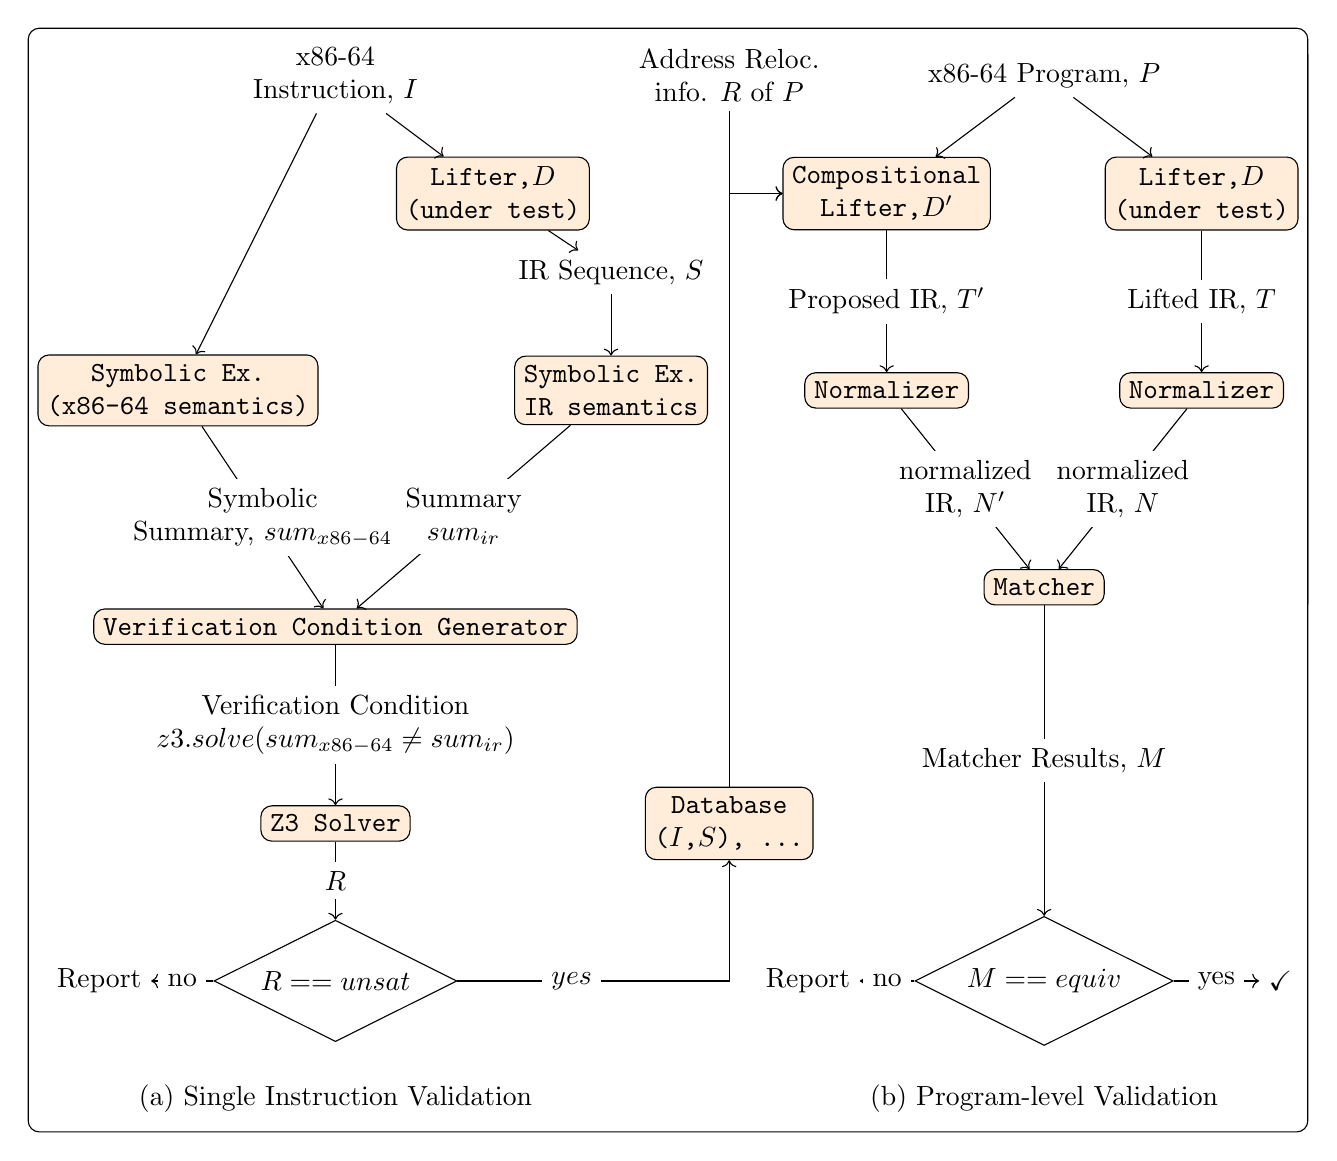
\begin{tikzpicture}[%node distance=2.5cm,
every node/.style={fill=white}, align=center]
\tikzset{%
    %>={Latex[width=2mm,length=2mm]},
    % Specifications for style of nodes:
    base/.style = {rectangle, rounded corners,
         text centered},
    process/.style = {base,  fill=orange!15, font=\ttfamily, draw=black},
    basic box/.style = {
        shape = rectangle,
        align = center,
        draw  = #1,
        %fill  = #1!25,
        rounded corners},
      header node/.style = {
        %Minimum Width = header nodes,
        font          = \strut\Large\ttfamily,
        text depth    = +0pt,
        fill          = white,
        draw},
      header/.style = {%
        inner ysep = +1.5em,
        append after command = {
            \pgfextra{\let\TikZlastnode\tikzlastnode}
            node [header node] (header-\TikZlastnode) at (\TikZlastnode.north) {#1}
            %node [span = (\TikZlastnode)(header-\TikZlastnode)] at (fit bounding box) (h-\TikZlastnode) {}
        }
      },
}
\def\blockhdist{2cm}
\def\blockvdist{1.5cm}
\def\phasehdist{8cm}

%%%%%%%%%%%%%%% PHASE I
\node (instr)          [base]  {\ISA\\ Instruction, $I$};
\node (SIVmcsema)   [process, below of=instr, yshift=-0.5cm, 
xshift=\blockhdist]  {Lifter,$D$\\(under test)};
\node (irseq)          [base,below of=SIVmcsema, xshift=\blockvdist]  {IR 
Sequence, $S$};
\node (instrSymEx)   [process, below of=instr, yshift=-2*\blockvdist, xshift=-\blockhdist] {Symbolic Ex.\\(\ISA semantics) };
\node (irSymEx)   [process, below of=irseq, yshift=-0.5cm] {Symbolic Ex.\\IR semantics};
\node (proofGen)   [process, below of=instr, yshift=-4*\blockvdist] 
{Verification Condition Generator};
\node (solver)   [process, below of=proofGen, yshift=-\blockvdist] {Z3 Solver};
\node (decide1)     [draw, below of=solver, yshift=-1cm, diamond, aspect=2]  {$R == unsat$};
\node (report1)       [left of=decide1, xshift=-\phasehdist/4]  {Report};
\node (caption1)     [below of=solver, yshift=-2.5cm] {(a) Single Instruction
    Validation};

\draw[->]             (instr) -- (SIVmcsema);
\draw[->]             (SIVmcsema) -- (irseq);
\draw[->]     (instr) -- (instrSymEx);
\draw[->]     (irseq) -- (irSymEx);
\draw[->]     (instrSymEx) -- node {Symbolic\\Summary, $sum_{\ISA}$} (proofGen);
\draw[->]     (irSymEx) -- node {Summary\\$sum_{ir}$ } (proofGen);
\draw[->]     (proofGen) -- node {Verification Condition\\$z3.solve(sum_{\ISA} 
\ne 
sum_{ir})$} (solver);
\draw[->]     (solver.south) -- node {$R$} (decide1.north);
\draw[->]     (decide1.west) -- node {no} (report1);

%%%%%% Store
\node (store)     [process, right of=solver, 
xshift=\phasehdist/2]{Database\\({$I$,$S$}), \dots};
\draw[->]       (decide1.east) -| node[xshift=-2cm] {$yes$} (store.south);


%%%%%%%%%%%% PHASE II
\node (start)             [base,right of=instr, 
xshift=\phasehdist]                       {\ISA Program, $P$};
\node (compd)             [process, below of=start, yshift=-0.5cm, 
xshift=-\blockhdist]          {Compositional\\Lifter,$D^\prime$};
\node (mcsema)             [process, below of=start, yshift=-0.5cm, 
xshift=\blockhdist]          {Lifter,$D$\\(under test)};
\node (normalizer1)             [process, below of=compd, yshift=-\blockvdist]   {Normalizer};
\node (normalizer2)         [process, below of=mcsema, yshift=-\blockvdist]   {Normalizer};
\node (matcher)     [process, below of=normalizer2, yshift=-\blockvdist, 
xshift=-\blockhdist]   {Matcher};
\node (decide2)     at (decide1 -| matcher) [draw,  diamond, aspect=2]  {$M == equiv$};
\node (caption2)     at (caption1 -| matcher) {(b) Program-level Validation};
\node (report2)       [left of=decide2, xshift=-\phasehdist/4]  {Report};
\node (fine)       [right of=decide2, xshift=\phasehdist/4]  {\checkmark}; 
 
\draw[->]             (start) -- (compd);
\draw[->]             (start) -- (mcsema);
\draw[->]     (compd) -- node {Proposed IR, $T^\prime$} (normalizer1);
\draw[->]     (mcsema) -- node {Lifted IR, $T$} (normalizer2);
\draw[->]     (normalizer1) -- node {normalized\\IR, $N^\prime$} (matcher);
\draw[->]     (normalizer2) -- node {normalized\\IR, $N$} (matcher);
\draw[->]     (matcher) -- node {Matcher Results, $M$} (decide2);
\draw[->]     (store.north) |-  (compd.west);
\draw[->]     (decide2.west) -- node {no} (report2);
\draw[->]     (decide2.east) -- node {yes} (fine);

%% Reloc info
\node (reloc)             [base,right of=instr, 
xshift=\phasehdist/2]                       {Address Reloc. \\ info. 
$R$ of $P$};
\draw[->]       (reloc.south) |-  (compd.west);

%% Outter box
\begin{scope}[on background layer]
\node[fit = (compd)(mcsema)(start)(matcher), basic box = black,] (Phase1) {};
    \node[fit = (compd)(mcsema)(start)(matcher)(instr)(solver)(irseq)(instrSymEx)(irSymEx)(caption1)(caption2), basic box = black,] (Overview) {};
\end{scope}

\end{tikzpicture}
\caption{Overview diagram of the \tv framework}\label{fig:overview}
\end{figure*}

% \tikzset{
%     database/.style={
%         path picture={
%             \draw (0, 1.5*\database@segmentheight) circle [x radius=\database@radius,y radius=\database@aspectratio*\database@radius];
%             \draw (-\database@radius, 0.5*\database@segmentheight) arc [start angle=180,end angle=360,x radius=\database@radius, y radius=\database@aspectratio*\database@radius];
%             \draw (-\database@radius,-0.5*\database@segmentheight) arc [start angle=180,end angle=360,x radius=\database@radius, y radius=\database@aspectratio*\database@radius];
%             \draw (-\database@radius,1.5*\database@segmentheight) -- ++(0,-3*\database@segmentheight) arc [start angle=180,end angle=360,x radius=\database@radius, y radius=\database@aspectratio*\database@radius] -- ++(0,3*\database@segmentheight);
%         },
%         minimum width=2*\database@radius + \pgflinewidth,
%         minimum height=3*\database@segmentheight + 2*\database@aspectratio*\database@radius + \pgflinewidth,
%     },
%     database segment height/.store in=\database@segmentheight,
%     database radius/.store in=\database@radius,
%     database aspect ratio/.store in=\database@aspectratio,
%     database segment height=0.1cm,
%     database radius=0.25cm,
%     database aspect ratio=0.35,
% }


\section{Single \ISA Instruction Validation}
\section{Preliminaries}
\label{sec:prelim}

In this section, we provide background on various pieces of our work:
(i) The binary lifter under test, McSema, (ii) The formal \ISA semantics, and
(iii) The formal \LLVM semantics.

\paragraph{McSema}\label{par:mcsema} \mcsema~\cite{McSema:Recon14} is the most
mature, well tested, open-source lifter to raise binaries from \ISA
instructions to LLVM bitcode.  At a high-level, \mcsema is split into two
parts: (a) frontend, and (b) backend. The frontend is responsible for parsing,
loading, and disassembling a binary and exports an interface to the backend to
query for the required information, e.g., the defined symbols, sizes of
various binary sections, instruction listings etc. The backend then uses this
information and Remill~\cite{Remill} library to lift the individual
instructions. McSema supports multiple different frontends with IDA Pro being
the most robust, and supported option.

Conceptually, the backend implementation of \mcsema is fairly straightforward:
\mcsema exposes all of architecture state, i.e., the program registers,
conditional flags, and program memory, through an LLVM \emph{struct}, aptly
named \Mcstate. 
Member fields
of the structure correspond to every register (register name, not a physical
register) and flags that can be used during the execution of the program. Instructions
operating on the stack must retrieve the current top of stack from the
appropriate member field (corresponding to \reg{rsp}) in the structure.
\mcsema simply scans through the disassembly of the binary
and lifts each instruction one by one, emitting code to read and update the
members of \emph{state} as defined by the instruction semantics. In essence,
the code lifted by \mcsema simply \emph{simulates} the binary in \LLVM.

%The main idea behind \mcsema lies in the simulation of the original binary,
%which in turns requires architectural state and memory of the target
%processor. There is no explicit stack by default.  To simulate state of the
%processor, an LLVM structure type called \emph{state} is used. Member fields
%of the structure correspond to every register (register name, not a physical
%register) that can be used during the execution of the program. Instructions
%operating on the stack must retrieve the current top of stack from the
%appropriate member field (corresponding to \reg{rsp}) in the structure.
%%\todo[inline]{Unclear: Since structure only holds registers, say which
%%register is used to retrieve "current top of stack."}
%\mcsema  performs decompilation of the binary code by translating the machine
%instructions to operations on this \emph{state} structure, according to the
%machine specification. This lifting process works by translating each assembly
%instruction in the procedure into an IR sequence,  which explicitly specifies
%how it affects the machine's memory and registers, including the flags.
%\paragraph{\ISA \& LLVM formal semantics}
%The present work needs the formal
%semantics of \ISA and LLVM, which we borrowed from~\cite{DasguptaAdve:PLDI19}
%and~\cite{LLVMSEMA} respectively. Both semantics are developed using
%\K~\cite{k-primer-2013-v32}\cmt{\url{http://kframework.org}}, which is a
%framework for defining formal language semantics.

\paragraph{K-Framework}\label{par:k} The presented work needs the formal
semantics of \ISA and LLVM, which we borrowed from~\cite{DasguptaAdve:PLDI19}
and~\cite{LLVMSEMA} respectively (and described next). Both semantics are developed using
\K~\cite{k-primer-2013-v32}\cmt{\url{http://kframework.org}}, which is a
framework for defining formal language semantics. Given a syntax and a
semantics of a language, \K automatically generates a parser, an interpreter, 
a symbolic execution engine, as well as
formal analysis tools such as model checkers and deductive program verifiers,
at no additional effort. Using the interpreter, one can test their
semantics immediately, which significantly increases the efficiency of
semantics developments. Furthermore, the formal analysis tools
facilitate formal reasoning about the given language semantics.  This
helps both the applicability of the semantics and in the
engineering the semantics itself.

\paragraph{\ISA Formal Semantics} Our work uses the state-of-the-art \ISA
semantics developed by Dasgupta et al.~\cite{DasguptaAdve:PLDI19}, which
presents the most complete and thoroughly tested formal semantics of x86-64 to
date, and faithfully formalizes all non-deprecated, sequential
user-level instructions of x86-64 Haswell instruction set architecture.
This totals to 3155 instruction variants, corresponding to 774 mnemonics.
Their semantics are fully executable, and includes a symbolic execution engine
automatically generated by \K framework
%
    \footnote{Given a syntax and a semantics of a language, \K automatically
    generates a parser, an interpreter, a symbolic execution engine, as well
    as formal analysis tools such as model checkers and deductive program
    verifiers, at no additional effort.}.
%

\paragraph{\LLVM Formal Semantics} We use the LLVM formal semantics as defined
in \K~\cite{LLVMSEMA}, which models LLVM types (integers, composite arrays and
structs, corresponding pointers), the \texttt{getelementptr} instruction (used
to compute the address of an element nested within a composite),  integer
arithmetic \& comparison operators, memory operations (\texttt{load},
\texttt{store}, and \texttt{alloca}), control flow instructions for
unconditional and conditional branches, as well as function calls and returns.
However, the semantics does not support: floating point, vector types, and
most LLVM intrinsic functions and therefore we cannot validate the \tv for
such instructions.  This is a limitation of the available LLVM semantics, and
not a limitation of our work.

.
%\todo[inline]{The last 2 sentences are nice, but could be dropped if space is tight.}
%\todo[color=yellow]{These two semantics are two of the most
%    important building blocks. Can we make them top-level paragraphs?}
%\paragraph{\ISA Semantics} \todo{These two semantics are two of the most
%important building blocks. Can we make them top-level paragraphs?}
%The formal model~\cite{DasguptaAdve:PLDI19}
%presents the most complete and thoroughly tested formal semantics of x86-64 to
%date, which faithfully formalizes all the  non-deprecated, sequential
%user-level instructions of the x86-64 Haswell instruction set architecture.
%This totals 3155 instruction variants, corresponding to 774 mnemonics.  The
%semantics is fully executable, and comes with an
%automatically generated symbolic execution engine (thanks to the \K framework),
%which we leverage in this work.
%
%\paragraph{LLVM Semantics} The formal semantics of \LLVM is provided by
%~\cite{LLVMSEMA}, which models  various LLVM types (like integer types,
%    composite array and struct types, the  corresponding pointer types, and the
%    \texttt{getelementptr} instruction used to compute the address of an element nested
%    within a composite type),  integer arithmetic \& comparison operators,
%  memory operations (like \texttt{load}, \texttt{store}, and \texttt{alloca}), 
%  control flow instructions
%  for unconditional and conditional branches, as well as function calls and
%  returns. The current version of the semantics does not support floating point
%  or vector types and most LLVM intrinsic functions, which constrains our experiments
%  but does not affect the overall approach proposed and evaluation in this work.
%  \todo{Check last sentence.}

%\paragraph{Stoke Libraries}\label{par:stoke} Stoke~\cite{Stoke2013} is a
%stochastic superoptimizer and program synthesizer for the x86-64 instruction
%set.  The project comes with many useful libraries to (1) query interesting
%properties of \ISA instructions (like type, size, inputs \& outputs etc.),
%(2) disassemble \ISA programs, and (3) analyze  \ISA programs to infer
%properties related to control- \& data-flow. We make use of these in our
%work.
%
%The rest of this paper is organized as follows: we discuss our \siv
%in~\ref{sec:siv}, and then move on to show how we use the validated sequences of
%IR instructions to construct a \emph{\compd} and use it to for \plv
%in~\ref{sec:plv}. Finally, we show the effectiveness of our developed techniques
%through our evaluation in~\ref{sec:eval}.

\section{\ISA Program-Level Validation}
\subsection{Compositional Decompiler}
\subsection{Normalizer}
\subsection{Matcher}

\chapter{Formal Semantics of \ISA User-Level ISA}\label{sec:results}
The equivalence checker being parametric on the semantics of source (\ISA) and target (LLVM) languages of decompilation, one of the important steps towards the goal is to define these semantics. In this section, we will discuss our published contribution~\cite{DasguptaAdve:PLDI19} is coming up with the most complete and thoroughly tested formal
semantics of x86-64 to date.


\section{Challenges in Formalizing \ISA}
\label{sec:challenges-in-formalizing-x86}
The \ISA instruction set architecture (ISA) is one of the most complex and widely used ISAs on servers and desktops, and ensuring the correctness of the \ISA binary code is important.
%
Completely formalizing the semantics of \ISA, however, is challenging especially due to the complexity and the sheer number of instructions that are informally specified in approximately 3,000-page standard~\cite{IntelManual}.
% In addition to the sheer number of instructions to be specified,
% % and the ambiguity of the informal standard document to consult,
% the following aspects make it challenging to completely specify the formal semantics of \ISA.

\paragraph{Size and Complexity:}
%
\SC{The \ISA ISA has a large number of instructions, partly because of a large number of complex instructions and partly because it keeps most of the legacy and deprecated instructions ($\sim$ \Xmmx{}+) for the sake of backwards compatibility.}
It consists of \totalIntel{} mnemonics, and each mnemonic admits several variants, depending on the types (i.e., register, memory, or constant) and the size (i.e., the bit-width) of operands.

\paragraph{Inconsistent Instruction Variants:}
%
Some variants have divergent behaviors more than the difference of their type and size. For example, \instr{movsd}, one of the 128-bit SSE instructions, has very different behaviors depending on whether the type of the source operand is register or memory; it clears the higher 64 bits of the target register only when the source type is memory.
Indeed, we revealed bugs in other semantics due to their incorrect generalization of the variants' behavior.

\paragraph{Ambiguous Documentation:}
%
The \ISA reference manual informally explains the instruction behaviors, leaving certain details unspecified or ambiguous, which required us to consult with an actual processor implementation to clarify such details.
%
Completely formalizing the vast number of instructions with carefully identifying all the corner cases from the informal document, thus, is highly non-trivial.


\paragraph{Undefined Behaviors:}
%
The \ISA standard also admits undefined behaviors that are implementation-dependent.
Many instructions (\undefIntel{}\footnote{\label{note1}These numbers are obtained by parsing the official manual ``Volume 2: Instruction Set Reference'' and cross checked with projects~\cite{Stoke2013, Felix} investing similar efforts.} out of \totalIntel{} mnemonics) have undefined behaviors: their output values of the destination register or the \reg{rflags} register are undefined in certain cases.
That is, the processor is free to choose any behavior in the undefined case.


Many existing semantics, however, simply ``define'' the undefined behaviors by
following a specific behavior taken by a processor implementation.
This approach is problematic because they do not capture all possible behaviors of different processor implementations.
Indeed, we found discrepancies between existing semantics in specifying the undefined behaviors, where different semantics are valid only for different groups of processors.
That is, such semantics are not adequate to formally reason about universal properties (e.g., portability) of a program that need to be satisfied for all standard-conforming processors.
%
For example, the parity flag \reg{pf} is undefined in the logical-and-not instruction \instr{andn}, where the processor implementation is allowed to either update the flag value (to 0 or 1), or keep the previous value.
We found, e.g., that Remill~\cite{Remill} updates the flag with 0, whereas Radare~\cite{Radare2} keeps it unmodified.
Identifying and faithfully specifying all the undefined behaviors, thus, are desirable but challenging.

\SC{In our semantics, we faithfully modeled the undefined value as a unique symbol (called \s{undef}) whose value is nondeterministically decided each time within the proper range.}
These nondeterministic values are enough to capture and formally reason about all possible behaviors of the instructions for different processors (and even any future, standard-conforming processor).

\section{Existing Semantics for \ISA}

To date, to the best of our knowledge, despite several explicit attempts~\cite{Heule2016a,Goel:FMCAD14,Goel:ProCoS17} and other related systems~\cite{Leroy:2009,Remill,TSL:TOPLAS13,Hasabnis:ASPLOS16,Hasabnis:FSE16},
no \emph{complete} formal semantics of \ISA exists that can be used for formal reasoning about x86 binary programs.
%
Heule~\etal \cite{Heule2016a} presented a formal semantics of \ISA, but it covers only a fragment ($\sim$\strataPerc{}) of all instructions; as the authors of \cite{Heule2016a} candidly admitted, their synthesis methodology proved insufficient to add the remaining instructions primarily due to limitations of the underlying synthesis engine. 
%
Moreover, their semantics misses certain essential details~\cite{DasguptaAdve:PLDI19}.
% and it has not been demonstrated how to use their semantics to formally reason about the functional correctness of the \ISA binary.\footnote{Although they provide a tool that can extract SMT formulae describing each instruction's behavior from their semantics, we found errors in their tool and thus the generated SMT formulae. Also, most of the SMT solvers are not designed to support rich reasoning principles.}
% natively support all the reasoning principles of the full-fledged proof assistants.}
% for the general purpose formal reasoning.}
%
% it is not clear how to lift their semantics to the full-fledged theorem prover to be able to reason about the full functional correctness of the \ISA binary.
% Although it can provide the semantics in the form of the SMT formulae, the SMT solver 
%
Goel~\etal~\cite{Goel:FMCAD14,Goel:ProCoS17}, on the other hand, specified a formal semantics in the \SC{ACL2} proof assistant~\cite{ACL2:Kaufmann2000}, allowing to reason about functional correctness, but their semantics covers only a small fragment ($\sim$\goelPerc{}) of all user-level instructions.
%\Comment{Section 2 says they had only 191 unique opcodes, which is only about 20\%, and even less if you include system instructions. Which is correct?}
%
There also have been several attempts~\cite{Angr1,BAP:CAV11,Radare2,Hasabnis:FSE16} to \emph{indirectly} describe the \ISA semantics, where they define an intermediate language (IL), specify the IL semantics, and translate \ISA to the IL.
This indirect semantics, however, may not be general enough to be used for different types of formal analyses, since the IL might be designed with specific purposes in mind, not to mention that the translation may miss certain important details of the instruction behaviors.
%
\section{Overview of the Approach}
\label{sec:Approach:Overview}

Briefly, our approach is as follows.
%
We first defined the machine configuration and underlying infrastructure in the \K framework, in order to define, execute and test the \ISA semantics.
%
\SC{To leverage previous work as much as possible, we took the semantic rules of all the instructions supported in Strata~\cite{Heule2016a}, which amounts to about 60\% of the instructions in scope, in the form of SMT formulas.}
%
We corrected, improved or simplified many of the baseline rules.
%
We then translated these SMT formulas from Strata into \K rules using a script, and tested the resulting rules by comparing with the Strata rules using Z3.
%
These steps give us a validated initial set of semantic rules in \K for about 60\% of the target instructions (our ``baseline'' set).

We attempted to extend the stratification approach in Strata to define additional rules automatically, in two ways: (i) augmenting their base set \s{B}, and (ii) constraining the search space manually using knowledge of instruction behaviors.  Both these attempts failed; they worked only for a few instructions, but in general, we found them to be impractical. Specifically, we added $58$ base instructions to the base set, and learned the semantics of $70$ new instructions, which are variants of the added  instructions, in $20$ minutes, but no more even after we kept running for two days. Also, we tried constraining the search space by manually populating it with relevant instructions. The lesson we learned from these experiments is, getting the right set of base instructions or a constrained search space for a complex instruction need an insight about the semantics of that instruction itself. We found that the effort to extract such information from the manual is about the same  as manually defining that instruction.


%\Comment{SANDEEP: Please check this last sentence and fix / improve.}

We then manually added \K rules for the remaining 40\% of the target instructions by systematically translating their description of the Intel manual into \K rules, in some cases cross-referencing against semantics available in Stoke.
%
The outcome was a complete formal specification of user-level \ISA in \K.

We validated this semantics in three ways:
%
First, we use the \K interpreter to execute the semantics of \emph{each} instruction for 7,000+ test inputs (each input is a processor state configuration) and compared the output directly with the hardware behavior for the same instruction.
%
Second, we repeated this experiment using the applicable programs in the \SC{GCC C-torture tests~\cite{CTORTURE}}.  % (\TortureInclude{} out of \TortureTotal{} tests).
%
Third, we compared against the semantics defined in the Stoke project for about 330 instructions that were omitted in Strata (thus not included in our baseline), using an SMT solver.

These validation experiments uncovered bugs~\cite{BugIntel,BugStoke983,BugStoke986} in the Intel manual, in Strata's simplification rules, and in the Stoke semantics.  All these bugs were reported to the respective authors, and most have been acknowledged and some have been fixed. Following is the brief summary of inconsistencies we found during the validation experiments.

\paragraph{Inconsistencies Found in the Intel Manual}
According to the manual, the semantics of \instr{vpsravd} \instr{\%xmm3,} \instr{\%xmm2,} \instr{\%xmm1} seems to depend on the lower $100$ bits of \reg{xmm3}, whereas the actual hardware execution suggests that it should depend on the lower $128$ bits. Similar inconsistencies are found in instructions with mnemonics \instr{vpsllvd}, \instr{vpsllvq}, \instr{vpsravd}.
Also, we found misleading typos related to instructions with opcodes \instr{vpsravw}, \instr{vpsravd}, \instr{vpsravq}, \instr{packsswb}.    
All these findings were reported and acknowledged by Intel as issues in the manual~\cite{BugIntel}.

\paragraph{Inconsistencies Found in \Strata's Simplification Rules}
While testing the instructions specifications borrowed from \Strata, we found inconsistent behaviors with the actual hardware. Moreover, the inconsistencies were discovered in the formulas of floating-point instructions. This is not surprising because \Strata models the floating-point instructions as \uif{} which cannot be executed or tested on hardware. Their semantics are executable in our definition though, and thus we were able to test them thoroughly. Note that Strata generates the formulas for these instructions by symbolically  executing  the corresponding learned  instruction sequences followed by a formula simplification pass. Therefore, errors in those formulas can be due to bugs either in the symbolic execution engine or in the simplification stage. Our testing shows that the second is true with the following evidence.
The simplification rule \s{add\_double(A, 0) == A} does not hold for \s{A = $-0.0$}. Same for \s{add\_single}. These were reported~\cite{PC1}.
Also, the simplification rule \s{sub\_double(A, A) == 0} does not hold for \s{A = $NaN$}.  Same is true for \s{sub\_single}. We found this bug in the  branch of Stoke which is used in \Strata. But this has been already fixed in the latest \Stoke branch.

\paragraph{Inconsistencies Found in \Stoke}

First, for instructions like \instr{addsubpd \%xmm1, \%xmm2} , the order of addition and subtraction specified by \Stoke is opposite to the one specified in the Intel Manual. Same is true with the mnemonic \instr{addsubps}. (Found in $12$ instruction variants.)

Second, the instruction \instr{pslld \%xmm1, \%xmm2} implements a logical left shift of packed data by a count specified in \reg{xmm1}. \Stoke's specification vectorized the operand \reg{xmm1} which is incorrect according to the manual. Similar issues were found in instructions implementing the logical right shift operations on packed data. (Found in  $18$ instructions.)

Third, \instr{cvtsi2sdl} \instr{\%eax,} \instr{\%xmm1} and \instr{vcvtsi2sdl} \instr{\%eax,} \instr{\%xmm0,} \instr{\%xmm1} are respectively SSE- and AVX-versions of the instruction to  convert a double-word ($32$-bit) integer to a scalar single-precision floating-point value. According to the manual, in the AVX-version,  the  destination bits $127-64$ of the  register \reg{xmm1} are updated to the corresponding bits in the first source operand \reg{xmm0}. This  is in contrast to the SSE-version of the instruction where the destination bits $127-64$ should remain unmodified. \Stoke specifies the semantics of the AVX-version similar to the SSE-version, which is incorrect.  (Found in $4$ instruction variants.)

Finally, some instructions, like \instr{imulb \%al}, which drive flag registers to an undefined state are not modeled correctly in \Stoke.    (found in $8$ instruction variants)

All these errors were reported and confirmed~\cite{BugStoke983,BugStoke986}.

\vspace{4pt}
Moreover, we illustrate the potential of our semantics to be used for formal analyses such as deductive program verification and program equivalence checking. For example, following are the three applications that we demonstrated:

\paragraph{Program Verification} To demonstrate that our semantics can be used to verify
x86-64 programs, we use the x86-64 verifier to prove the
functional correctness of the sum-to-n program. The functional correctness
property, which is $return-value = \sum_1^N n = N (N + 1) / {2}$ is specified as reachability specifications, essentially a pair of pre- and post-conditions for the function computing the sum-to-n.

\paragraph{Symbolic Execution to find Security Vulnerability}
\K automatically derives a correct-by-construction symbolic execution engine from the given semantics.
Being instantiated with our semantics, the engine can be used to symbolically execute and explore all possible paths in the given \ISA program.
We demonstrated how this capability can be used to find a  security vulnerability. We took a known security vulnerability using a code snippet of the HiStar~\cite{HiStar:2006} kernel. Using symbolic execution, we derive a path condition which can trigger the  vulnerability along with the triggering inputs.

\paragraph{Translation Validation of Optimizations}
\K also provides a program equivalence checker that can be used for the translation validation of compiler optimizations.
We derived an \ISA program equivalence checker from our semantics and used it to validate different optimizations of \s{popcnt} program which counts the number of set bits in the given input. We compiled the program with different optimizations: the GCC compiler optimizations (-O0, -O1, -O2, and -O3), and the Stoke super-optimization. We validated these optimizations by checking the equivalence between the optimized programs.


The \K framework also enables one to represent our semantics as SMT theories, which allows others to easily reuse our semantics for their own purposes.
\SC{%
    Indeed, we have translated our semantics to Stoke~\cite{completing-stock} which can serve as a drop-in replacement of Heule~\etal's semantics~\cite{Heule2016a} and can immediately benefit tools built on Stoke (e.g., \cite{Roessle:CPP19}).
}
%
% \paragraph{Artifacts}

Our formal semantics is publicly available at~\cite{x86-64-github}.



\chapter{Ongoing and Future Work: Translator-agnostic Translation
  Validation}\label{sec:future}

With the overall goal of  establishing faithfulness of binary lifters, we
propose to use \tv to validate the translation from binary to LLVM IR\footnote{However, we believe that the core techniques are
    applicable to other decompilers targeting mid-level (language-neutral) IRs}. As
mentioned earlier, we employed \K framework as the formalism medium to
represent the source and target language and in the process, defined the most
complete semantics of user-level \ISA using the framework. We proposed to
borrow a language-independent equivalence checking algorithm
\m{Keq}~\cite{TheoSAS19} that can be parameterized with the input and output
language semantics. 
%The algorithm needs, as input, the \syncps for establishing equivalence
%between binary and LLVM IR programs, which can be generated by the translator
%itself.  .

As mentioned in Section~\ref{sec:approach}, the notion of equivalence between
binary program and the lifted LLVM IR is formalized as a bi-simulation
relation~\cite{Sangiorgi:2011} between pairs of states of the two programs.
These program points, also referred to as \syncps, are generated by a proof generator and fed to the equivalence
checker as inputs. There are various ways a proof generator can generate these
\syncps each having different challenges and trade-offs.

\section{Translator-specific approaches to SYNCHRONIZATION POINT
  generation}\label{sec:TS} One approach to generate the \syncps is by
  instrumenting the translator itself. 
%
% and can
%be generated, by a proof generator,  as hints by analyzing the translator
%itself. 
The translator, being aware of which high-level IR instructions and control
points are emitted for each binary instruction, can accurately generate the
\syncps. Moreover, each \syncp is labeled with invariants over symbolic
variables, corresponding to input/output program states, in order to cover only
observably equivalent states. For each \syncp, the equivalence-checker checks
equivalence by delegating proof obligations to an SMT solver. Failure of a
proof obligation can be attributed to either a bug in the translator or  the
fact that the source and target programs are not equivalent in the first place.
We can rule out the second possibility because the source and target programs
are not selected arbitrarily but they are the actual input and output of a
translator, under test, and hence claimed to be equivalent by the translator
itself.

However, the above approach requires modifications of the translator to
generate the \syncp points and hence it may not be easily scalable to other
decompilers. 

Another approach is to analyze the source (\ISA) code and target (LLVM IR) code
of a particular translation  and infer the synchronization points.
We note that the analyzer has to take into account translators specific idioms
while analyzing the target code because different binary translators might use
different ways to lift the binary code in the target IR. We would demonstrate
the applicability of this approach by validating the translation of a realistic
decompiler like McSema~\cite{McSema:Recon14}

\section{Translator-agnostic approaches to SYNCHRONIZATION POINT
  generation}\label{sec:TA}

The fact that the proof generator is using translator generated hints or idioms used by the translator
to  generate the \syncps \& the associated  invariants,  makes it  translator specific and hence not applicable
uniformly across translators. We aim for a  binary-translator-agnostic proof
generator, which, indeed, makes the problem  even more challenging. We would
like to explore the following  approaches towards that goal.

\paragraph{\textbf{Data-driven \syncp generation}} This approach
is based on inferring the \syncps using test-runs. There are two
notables~\cite{Iman2005,DDEC:OOPSLA:2013} along this direction which
deals with checking equivalence between GCC~\cite{GCC} RTLs or x86 loops respectively.

Iman \etal~\cite{Iman2005} proposed an algorithm for solving the problem of
finding basic block and variable correspondence between two GCC RTL programs
compiled from the same source, but using different optimizations.  The essence
of their technique is interpretation of the two programs on random inputs and
comparing the histories of value changes for variables.  If the sequences of
value changes of two variables are the same, then the variables probably
correspond to each other, and the block in which the changes occur might also
correspond to each other. However, the paper candidly admits that they do not consider  generation of
verification invariants (VCs) at a point of correspondence or proving the VCs, hence it is difficult
to judge  its effectiveness in proving the equivalence of the candidate RTL
programs.  \cmt{ Moreover, the paper do not try to address any reordering
  transformation, that is any transformation that changes the order of
    execution of code, without adding or deleting any executions of any
    statement. Also, using random values results in poor code coverage which is
    detrimental to finding variable correspondence. We note that only the basic
    blocks \m{b1} and \m{b2}, which are covered by the same test input run in
    original and optimized versions respectively, can be the candidate for
    correspondence.}   


%DDEC~\cite{DDEC:OOPSLA:2013} uses a combination of static analysis and
%data-driven inference for constructing simulation relations: Static analysis is
%used to determine the program locations of \syncps and the live
%variables while the constraints between variables are inferred from execution
%traces. 


Rahul \etal~\cite{DDEC:OOPSLA:2013} presented ``data-driven equivalence
checker'' (DDEC) to check equivalence of two x86 loops which uses data-driven
inference in order to guess candidate simulation relations\footnote{A 
  simulation relation can be roughly defined to consist of a pair of program cutpoints, which breaks two
    loops into a set of pairs of loop-free code fragments and  linear
    equalities as invariants to hold at those cutpoints.}. Their approach does
    not assume any knowledge about the optimization performed while determining
    those simulation relations. The candidate simulation relations are checked
    using an SMT solver to determine equivalence of the loops. The cutpoints
    are chosen where the corresponding memory states agree on the largest
    number of values. The equality conditions   at cutpoint is determined by
    using standard linear algebra techniques over the values of live variables
    recorded by inserting instrumentation. Moreover, DDEC is sound; a lack of
    test coverage may cause equivalence checking to fail, but it cannot result
    in the unsound conclusion that two loops are equivalent when they are not.
    \cmt{However, while DDEC is trying to prove that two x86 loops are
      equivalent, the proof obligation might fail because  of one or more of
        the following reasons: (1 ) If satisfactory cutpoints are not found,
            (2) If spurious equality relationships are produced as invariants,
            (3) There is a bug in the translator, and (4) The target and the
              rewrite are not equivalent in the first place. The attribution of
              failure reason seems non-trivial and could affect fully automatic
              application of the approach.}   

%Our proposed approach is based on the insight that a sound guess of
%synchronization points do not result in proving two programs equivalent when
%they are not (false positives). Indeed, they might produce false negatives.
%Having said that, 

Our proposed approach is based on the insight that
given  \ISA and translated LLVM programs, we might compile
the LLVM program to binary and use the data-driven
approach~\cite{DDEC:OOPSLA:2013}, mentioned above, to extract guesses of
\syncps. Next, we can map the \syncps back to the IR level and employ the equivalence
checker \m{Keq} to prove the equivalence of the resulting LLVM IR and the
original binary using the \syncp guesses. We note that, an incorrectly guessed, but sound \syncp will never result in proving two programs equivalent when
they are not (false positives) and hence we do not have to trust the compilation back-end.

%However, we do not want to add the compilation in our trust base and
%hence we can map the \syncps back to the IR level and employ the equivalence
%checker \m{Keq} to prove the equivalence of the resulting LLVM IR and the
%original binary using the \syncp guesses. 
However, these \syncp, being
data-driven guesses, may lead to failing the proof obligations for reasons
other than a translation error. For example, the proof might fail if the
spurious invariants are generated or the \syncps are not sufficient, and it is
highly non-trivial, but an interesting research problem, to automatically
attribute the failure reasons. 

There is a trade-off between translator-specific and translator-agnostic proof
generator approaches. The \syncps generated by the former is accurate, leading
to trivial and automatic attribution of proof failure reason. On the other
hand, the \syncp guesses produced by the  translator-agnostic proof generator
has issues with automatic attribution  of the failure reasons. We envision
opportunities to exploit this trade-off by pruning off \syncp  guesses which a
translator specific proof generator will never generate. For
  example, the equivalence checker \m{Keq}~\cite{TheoSAS19} is used for
    validating the compilation pipeline and it uses compiler generated hints to
    prove equivalence. The underlying algorithm mandates three
%equivalence-checker \m{Keq}~\cite{TheoSAS19}, which employs a
%translator-specific proof generator  to validate compilation,  dictates three
broad categories of synchronization points which are necessary and sufficient
to prove equivalence, viz., entry points, exiting points (which also include
    points before callsites), and the rest of the points (including loop entry
      points and points after callsites). We may use this information to prune
    redundant \syncp guesses generated by a translator-agnostic  proof
    generator like DDEC~\cite{DDEC:OOPSLA:2013}.

\paragraph{\textbf{Learning \syncps}}

As discussed in Section~\ref{sec:ml}, there exist many recent
efforts~\cite{Jaffe:2018ICPC,Rosenblum2007,Rosenblum:2008,Rosenblum:2010,Rosenblum:2011,Bao:2014,Shin:2015}
in extracting various features (like meaningful variable names, compiler
    provenance, function entry points) using machine learning techniques which
are useful for binary analysis. Most notable is the novel technique presented
by Katz \etal~\cite{katz2018rnn}  for decompiling binary code snippets using a
model based on Recurrent Neural Networks. The model learns properties and
patterns that occur in source code and uses them to produce decompilation
output. 
%

The employed model is  a sequence-to-sequence model based on RNNs. The model
composed of two recurrent neural networks: an encoder, which processes the
input binary sequence, and a decoder, which creates outputs, the decompiled C
code. Further, the sequence-to-sequence model contains a hidden state, which
summarizes the entire input sequence. 
%
The training input contains of a large pair of strings representing the snippet
of source C code and the corresponding binary output, derived from open source
projects.  The snippets are preprocessed  by tokenizing each string  and
translating the resulting token list to a list of integers. Preprocessing also
produces a dictionary to map which integers correspond to which tokens in both
the higher-level and binary snippets.  The encoder layer of the RNN is trained
using the list of integers, derived from binary and the decoder layer is
trained using the corresponding list of integers, derived from C code.  During
training, the encoder-decoder modifies its internal state and does not provide
additional output. For testing, the test-binary snippets are translated into
lists of integers, which is then fed to the trained encoder-decoder model to
output a list of integers, which  is later turned into  a predicted higher-level C
translation using the dictionary  generated in the preprocessing step.
%
There evaluation results suggest that the technique  can be used to obtain a high level
syntactic structure of the code.
    
    
For an input binary and the high-level IR, translated by an arbitrary
decompiler, our goal is to learn the corresponding \syncp. Using a
straightforward  supervised-learning approach, we could frame the problem as:
To predict if an arbitrary pair of program points is a \syncp or not?
Such a supervised-learning formulation requires providing  many input code
snippets, correctly labeled with \syncps, as the training set in the first
place. Indeed, it is interesting to explore how to harvest the input corpus. 
 

Another way of inferring the \syncps is by using ``Trial and Error'', for which
Reinforcement Learning~\cite{Sutton:1998} seems to be a better choice to
explore. For the ``Trial and Error'' approach to work, there must be an
efficient way to find the error state, namely, the tried \syncp is non-valid.
With that, the goal of inferring all the corresponding \syncps of an input
output program pair can be defined solely in terms of some \emph{reward} given
on each selection. For example, for each selection of \syncp, a \emph{reward}
can be assigned using the number of values on which the corresponding memory
states agree on, when they are both tested using a random set of same  inputs.

We believe such learning techniques are promising for this problem and we would like to explore more on this in the proposed work.

\cmt{
Chen \etal~\cite{CLSS2015}
The second approach performs validation based on the basic blocks of the programs. This approach is widely applied in
the validation of optimizing compilers [8,9]. However, the basic-block validation is not suitable for validating static binary translators because the target addresses of indirect branches may not be resolved completely at static time, which implies that it may not be possible to build an accurate control flow graph from binary code. In contrast, we choose to perform validation based on individual instructions since per-instruction validation can help to detect the mistranslated instructions more accurately.


The notion of a certifying
compiler~\cite{Necula:2000,Pnueli:1998,Stepp:2011,Tristan:2011} is
significantly easier to employ than a formal compiler
verification~\cite{Leroy:2009}, in part because it is generally easier to
verify the correctness of the result of a computation than to prove the
correctness of the computation itself. 

}





%%%%%%%%%%%%%%%%%%%%%%%%%%%%%%%%%%%%%%%%%%%%%%%%%%%%%%%%%%%%%%%%%%%%%%%%%%%%%%%
% APPENDIX
%
%\appendix
%\include{apx}

\backmatter

%%%%%%%%%%%%%%%%%%%%%%%%%%%%%%%%%%%%%%%%%%%%%%%%%%%%%%%%%%%%%%%%%%%%%%%%%%%%%%%
% BIBLIOGRAPHY
%

%\bibliographystyle{IEEE_ECE}
\bibliographystyle{alpha}
% Put references in BibTeX format in thesisrefs.bib.
%\bibliography{thesisrefs}
\bibliography{bibs/decompilaion-validation,bibs/modeling-X86-semantics,bibs/references,bibs/bugs,bibs/k}


%%%%%%%%%%%%%%%%%%%%%%%%%%%%%%%%%%%%%%%%%%%%%%%%%%%%%%%%%%%%%%%%%%%%%%%%%%%%%%%
% AUTHOR'S BIOGRAPHY
% As of 10/03/2011, Author's Biography or Vita no longer accepted by Grad College

\end{document}
\endinput
